\documentclass[conference]{IEEEtran}
\usepackage{graphicx}
\usepackage{booktabs}
\usepackage{hyperref}
\usepackage{amsmath}
\usepackage{url}
\usepackage{cite}

\title{Indian Sign Language Recognition with Landmark Features:\\
Accuracy--Efficiency Tradeoffs Across Classical and Deep Models}

\author{Anurag Sharma\\
Department of Computer Science and Engineering,\\
JK Lakshmipat University, Jaipur, India\\
Email: bugruster@gmail.com}

\begin{document}

\maketitle

\begin{abstract}
We study isolated Indian Sign Language (ISL) word recognition on a school-collected dataset of 67 signs and 1{,}072 videos recorded with four native signers. Hand and upper-body landmarks from MediaPipe are converted into spatial and temporal features and classified with XGBoost, a CNN--LSTM model, and a compact Transformer. On our held-out test split the Transformer reaches 73.2\% accuracy, while XGBoost reaches 71.0\% with substantially lower training cost (15~min vs.\ 120~min) and faster inference (45~ms vs.\ 180~ms). The contribution is therefore not a single headline accuracy, but a practical accuracy--efficiency comparison on a publicly released ISL word set. Code and the dataset are available at \url{https://github.com/BugRuster/MJRIDK} and \url{https://www.kaggle.com/datasets/bugruster/isl-buggy-arn089}.
\end{abstract}

\begin{IEEEkeywords}
Indian Sign Language, gesture recognition, MediaPipe, XGBoost, CNN-LSTM, Transformer, assistive technology
\end{IEEEkeywords}

\section{Introduction}
Hearing-impaired communication in India relies heavily on Indian Sign Language (ISL), yet digital ISL tools remain sparse outside laboratory settings. Interpreter coverage is limited, and many existing recognition systems either depend on large public corpora that do not match local signing practice or require compute budgets that are awkward for school and clinic deployments.

This work addresses a narrow, concrete setting: isolated ISL word recognition from RGB video collected with students at Seth Anandi Lal Poddar Deaf, Dumb and Blind School in Jaipur. We release the resulting 67-word dataset on Kaggle, with accompanying code on GitHub, and compare three classifiers on the same landmark-derived features. The central empirical question is which model is worth deploying when accuracy, training time, and latency all matter.

Our objectives are therefore (i)~to document a reproducible collection protocol and feature pipeline, (ii)~to quantify the accuracy--efficiency tradeoff among XGBoost, CNN--LSTM, and a Transformer on this dataset, and (iii)~to state clearly where the pilot scale limits generalization.

\section{Related Work}
Early dynamic gesture systems leaned on Hidden Markov Models and carefully engineered features~\cite{starner1998}, while Support Vector Machines were widely used for static postures~\cite{huang1998}. Deep models later became dominant: CNNs for spatial appearance, LSTMs for temporal structure~\cite{hochreiter1997}, and Transformers for long-range attention~\cite{vaswani2017}. In practice, many recent sign-language pipelines extract skeletal landmarks first and then classify sequences, reducing sensitivity to clothing and background~\cite{lugaresi2019}.

For ISL specifically, INCLUDE introduced a large multi-signer corpus and the INCLUDE-50 subset used for rapid benchmarking, with reported top accuracy of 94.5\% on INCLUDE-50~\cite{sridhar2020}. CISLR expanded word-level ISL coverage to thousands of glosses~\cite{joshi2022cislr}, and ISLTranslate targets continuous translation pairs~\cite{joshi2023isltranslate}. These resources are valuable, but school-facing systems still need smaller, locally collected sets that match classroom vocabulary and recording conditions. Our dataset is intentionally smaller and more focused; we treat INCLUDE-50 numbers as context, not as a matched leaderboard.

\section{Method}
\subsection{System Overview}
Figure~\ref{fig:architecture} summarizes the pipeline: video preprocessing, MediaPipe landmark extraction, feature engineering, and classification. The four logical stages are input processing, feature extraction, classification, and gloss output.

\begin{figure}[t]
\centering
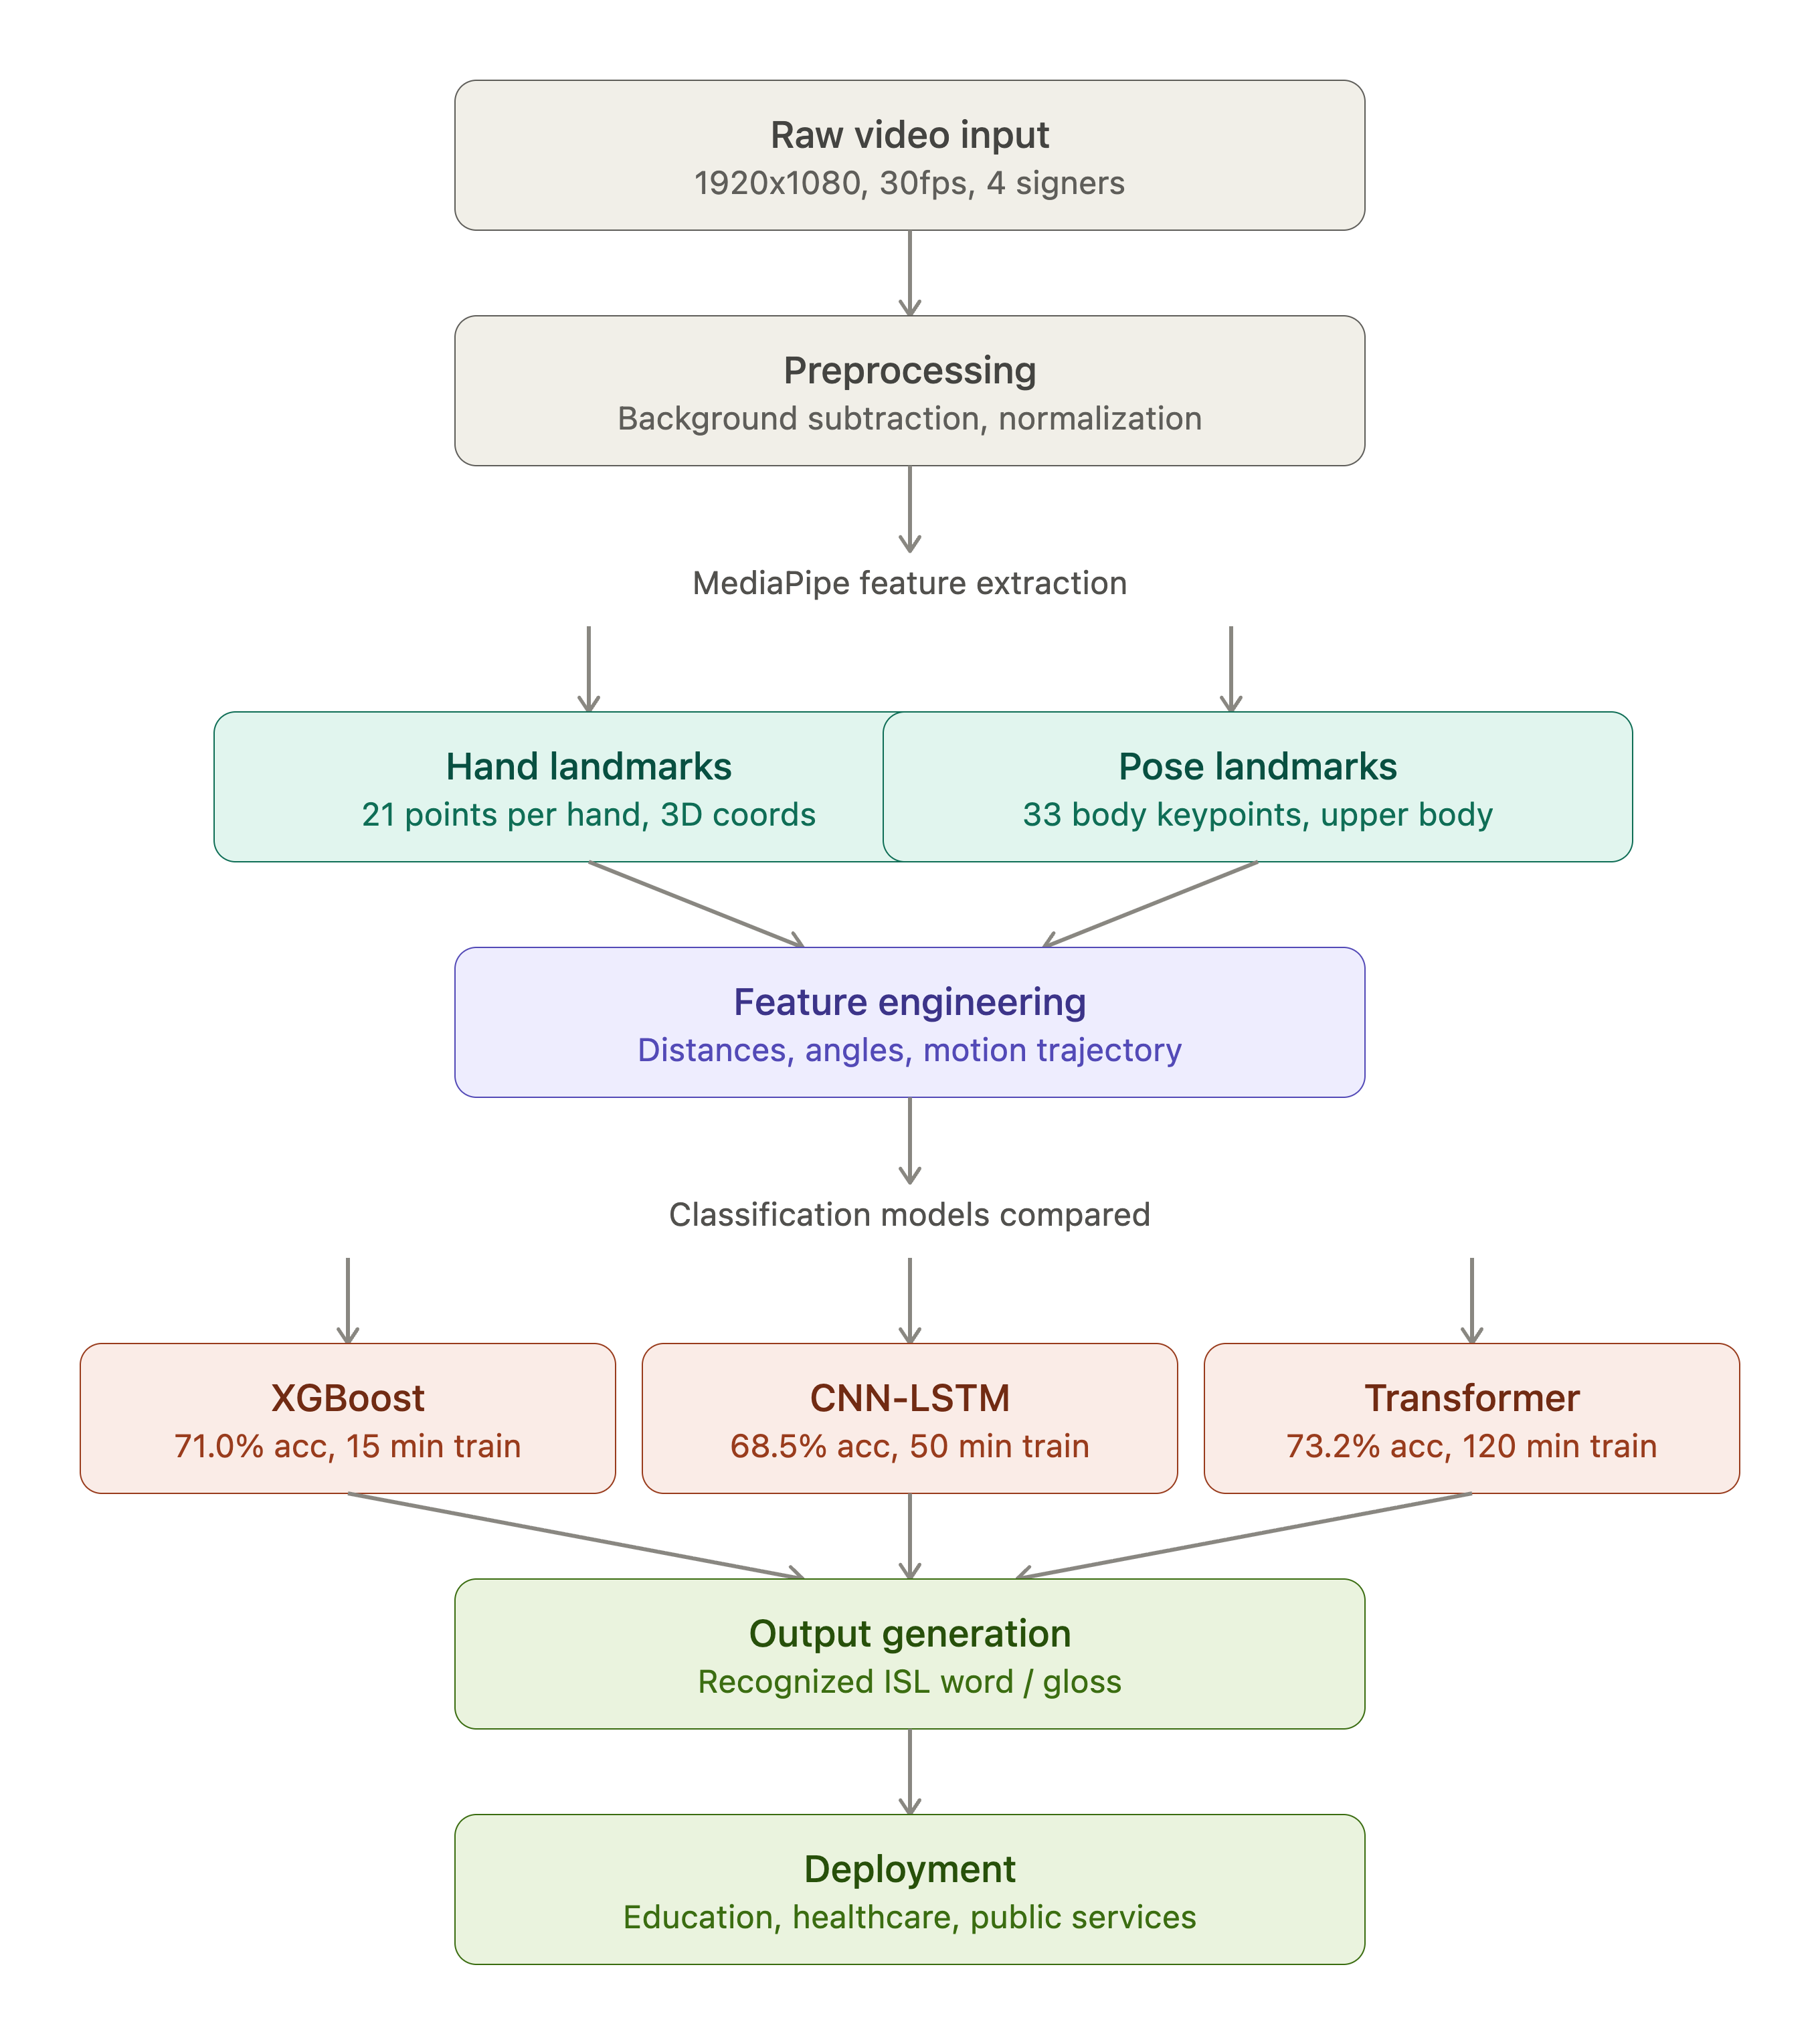
\includegraphics[width=0.92\linewidth]{isl_recognition_system_architecture.png}
\caption{ISL recognition pipeline used in this study. Parallel hand and pose landmarks feed a shared feature stage before the three classifiers.}
\label{fig:architecture}
\end{figure}

\subsection{Dataset}
\subsubsection{Collection}
Four native signers (two male, two female; ages 18--25) produced isolated signs under controlled indoor lighting against a neutral background. Videos were recorded at $1920\times1080$ and 30~FPS in H.264 MP4, typically lasting 2--5~seconds per clip. Each gloss was recorded multiple times to capture natural speed and hand-size variation.

\subsubsection{Composition}
Table~\ref{tab:dataset} lists the six semantic categories. The full set contains 67 words and 1{,}072 clips (16 clips per word on average). Code and the dataset are available at \url{https://github.com/BugRuster/MJRIDK} and \url{https://www.kaggle.com/datasets/bugruster/isl-buggy-arn089}.

\begin{table}[t]
\centering
\caption{Dataset composition by category}
\label{tab:dataset}
\begin{tabular}{@{}lccc@{}}
\toprule
Category & Words & Videos/word & Total \\
\midrule
Daily activities & 15 & 16 & 240 \\
Emotions & 12 & 16 & 192 \\
Colors & 10 & 16 & 160 \\
Animals & 8 & 16 & 128 \\
Numbers & 10 & 16 & 160 \\
Miscellaneous & 12 & 16 & 192 \\
\midrule
Total & 67 & -- & 1072 \\
\bottomrule
\end{tabular}
\end{table}

\subsubsection{Ethics}
Collection was conducted in collaboration with the partner school. Informed consent was obtained from participants (and guardians where required) before recording. Identifiers were removed from released filenames, and videos are shared for research use under the Kaggle dataset terms.

\subsection{Preprocessing and Features}
Frames are color-normalized and lightly denoised before landmark extraction. We use MediaPipe Hands and Pose~\cite{lugaresi2019}: 21 three-dimensional points per detected hand and 33 body keypoints with emphasis on the upper body. From these landmarks we compute pairwise distances, joint angles, and short-window motion trajectories. The resulting fixed-length feature vectors are the sole input to all three classifiers, so differences in Table~\ref{tab:acc} reflect the classifiers rather than mismatched front-ends.

\subsection{Classifiers}
Data were split 70/15/15 into train/validation/test with stratified sampling by gloss. Hyperparameters for XGBoost~\cite{chen2016} were selected by grid search on the validation set (depth~6, learning rate~0.01, 1000 estimators, subsample/colsample~0.8, L1/L2 regularization). The CNN--LSTM stacks 1-D convolutions over the feature sequence with a two-layer LSTM decoder. The Transformer uses a small encoder (two layers, four heads) over the same sequence with a linear classification head. All deep models were trained with early stopping on validation loss. We additionally report 5-fold cross-validation on the training pool for XGBoost stability.

\section{Results}
\subsection{Accuracy and Cost}
Table~\ref{tab:acc} reports test-set classification metrics. The Transformer is strongest on accuracy (73.2\%), followed by XGBoost (71.0\%) and CNN--LSTM (68.5\%). Table~\ref{tab:compute} shows why XGBoost remains attractive: it trains in about 15~minutes on our hardware, uses 2.3~GB memory, and infers in 45~ms, versus 120~minutes / 6.2~GB / 180~ms for the Transformer. For resource-constrained deployment the 2.2-point accuracy gap is often an acceptable trade for an $8\times$ reduction in training time and roughly $4\times$ faster inference.

\begin{table}[t]
\centering
\caption{Test-set performance on the 67-word ISL dataset}
\label{tab:acc}
\begin{tabular}{@{}lcccc@{}}
\toprule
Model & Acc. & Prec. & Recall & F1 \\
\midrule
XGBoost & 71.0\% & 0.72 & 0.70 & 0.71 \\
CNN--LSTM & 68.5\% & 0.69 & 0.68 & 0.68 \\
Transformer & 73.2\% & 0.74 & 0.72 & 0.73 \\
\bottomrule
\end{tabular}
\end{table}

\begin{table}[t]
\centering
\caption{Training and inference cost (same feature inputs)}
\label{tab:compute}
\begin{tabular}{@{}lccc@{}}
\toprule
Model & Train time & Memory & Inference \\
\midrule
XGBoost & 15 min & 2.3 GB & 45 ms \\
CNN--LSTM & 50 min & 4.8 GB & 120 ms \\
Transformer & 120 min & 6.2 GB & 180 ms \\
\bottomrule
\end{tabular}
\end{table}

\subsection{Comparison with Prior Datasets}
Table~\ref{tab:compare} situates our numbers next to published ISL benchmarks. The comparison is \emph{not} apples-to-apples: INCLUDE-50 uses a different vocabulary, more signers, and a different protocol~\cite{sridhar2020}. We include it to show scale and to avoid overstating our absolute accuracy. On our 67-word school set, the Transformer is the accuracy leader and XGBoost the efficiency leader.

\begin{table}[t]
\centering
\caption{Context against prior ISL resources (different datasets)}
\label{tab:compare}
\begin{tabular}{@{}lccc@{}}
\toprule
Work & Dataset & Vocab. & Acc. \\
\midrule
Sridhar et al.~\cite{sridhar2020} & INCLUDE-50 & 50 & 94.5\% \\
Joshi et al.~\cite{joshi2022cislr} & CISLR & $\sim$4.7k & -- \\
This work (Transformer) & School ISL & 67 & 73.2\% \\
This work (XGBoost) & School ISL & 67 & 71.0\% \\
\bottomrule
\end{tabular}
\end{table}

\subsection{Error Patterns}
Manual inspection of confusions suggests that near-identical handshapes and short motion differences account for roughly 45\% of errors, environmental factors (lighting, framing) about 29\%, and landmark or classifier failures the remainder. Similar gloss pairs within a category (for example, closely related emotion signs) dominate the confusion mass.

\subsection{Cross-Validation and Ablations}
Five-fold XGBoost accuracies were 70.8\%, 71.2\%, 70.5\%, 71.4\%, and 71.1\% (mean 71.0\%). Sample standard deviation is $\sigma=0.35$ percentage points; a $t$-based 95\% confidence interval for the mean is approximately $[70.6\%,\,71.4\%]$, indicating stable performance across folds (Table~\ref{tab:cv}).

\begin{table}[t]
\centering
\caption{XGBoost five-fold cross-validation}
\label{tab:cv}
\begin{tabular}{@{}cccc@{}}
\toprule
Fold & Acc. & F1 & Loss \\
\midrule
1 & 70.8\% & 0.71 & 0.32 \\
2 & 71.2\% & 0.70 & 0.31 \\
3 & 70.5\% & 0.71 & 0.33 \\
4 & 71.4\% & 0.72 & 0.30 \\
5 & 71.1\% & 0.71 & 0.31 \\
\midrule
Mean & 71.0\% & 0.71 & 0.31 \\
\bottomrule
\end{tabular}
\end{table}

Ablations on the XGBoost pipeline (Table~\ref{tab:ablation}) show that removing temporal features drops accuracy to 63.8\% ($-7.2$ points) and restricting to basic landmark coordinates drops it to 58.9\% ($-12.1$ points). Data augmentation contributes 5.7 points. Temporal geometry is therefore material on this vocabulary.

\begin{table}[t]
\centering
\caption{XGBoost ablation on engineered features}
\label{tab:ablation}
\begin{tabular}{@{}lcc@{}}
\toprule
Configuration & Acc. & $\Delta$ \\
\midrule
Full model & 71.0\% & -- \\
No augmentation & 65.3\% & $-5.7$ \\
No temporal features & 63.8\% & $-7.2$ \\
Basic coordinates only & 58.9\% & $-12.1$ \\
\bottomrule
\end{tabular}
\end{table}

\section{Limitations}
The dataset is a pilot: four signers from one institution cannot represent India's regional ISL variation. Splits are gloss-stratified rather than strictly signer-independent, so some signer-specific cues may leak across partitions. We evaluate isolated words only, not continuous signing. Absolute accuracies trail large curated benchmarks such as INCLUDE-50, which is expected given vocabulary differences and the smaller training pool.

\section{Conclusion}
On a publicly released 67-word ISL dataset, a compact Transformer yields the highest accuracy (73.2\%), while XGBoost remains competitive (71.0\%) at a fraction of the training and inference cost. The practical takeaway for school-scale assistive tools is to treat model choice as an accuracy--efficiency decision rather than a single-number race. Extending signer diversity, moving to signer-independent evaluation, and adding continuous recognition are the natural next steps.

\section*{Acknowledgments}
We thank Seth Anandi Lal Poddar Deaf, Dumb and Blind School, Jaipur, and the student participants who contributed recordings.

\bibliographystyle{IEEEtran}
\begin{thebibliography}{00}

\bibitem{starner1998}
T.~Starner, J.~Weaver, and A.~Pentland, ``Real-time American Sign Language recognition using desk and wearable computer based video,'' \emph{IEEE Trans. Pattern Anal. Mach. Intell.}, vol.~20, no.~12, pp.~1371--1375, 1998.

\bibitem{huang1998}
C.-L. Huang and W.-Y. Huang, ``Sign language recognition using model-based tracking and a 3D Hopfield neural network,'' \emph{Machine Vision and Applications}, vol.~10, pp.~292--307, 1998.

\bibitem{hochreiter1997}
S.~Hochreiter and J.~Schmidhuber, ``Long short-term memory,'' \emph{Neural Computation}, vol.~9, no.~8, pp.~1735--1780, 1997.

\bibitem{vaswani2017}
A.~Vaswani \emph{et al.}, ``Attention is all you need,'' in \emph{Proc. NeurIPS}, 2017, pp.~5998--6008.

\bibitem{lugaresi2019}
C.~Lugaresi \emph{et al.}, ``MediaPipe: A framework for building perception pipelines,'' arXiv:1906.08172, 2019.

\bibitem{chen2016}
T.~Chen and C.~Guestrin, ``XGBoost: A scalable tree boosting system,'' in \emph{Proc. ACM SIGKDD}, 2016, pp.~785--794.

\bibitem{sridhar2020}
A.~Sridhar, R.~G.~Ganesan, P.~Kumar, and M.~M.~Khapra, ``INCLUDE: A large scale dataset for Indian Sign Language recognition,'' in \emph{Proc. ACM Multimedia (MM)}, 2020, pp.~1366--1375.

\bibitem{joshi2022cislr}
A.~Joshi, A.~Bhat, P.~S, P.~Gole, S.~Gupta, S.~Agarwal, and A.~Modi, ``CISLR: Corpus for Indian Sign Language recognition,'' in \emph{Proc. EMNLP}, 2022, pp.~10357--10366.

\bibitem{joshi2023isltranslate}
A.~Joshi, S.~Agrawal, and A.~Modi, ``ISLTranslate: Dataset for translating Indian Sign Language,'' in \emph{Findings of ACL}, 2023, pp.~10466--10475.

\end{thebibliography}

\end{document}
